
\tikzset{eln/.style={midway, font = \Large,inner sep=2pt, outer sep=.30cm}}
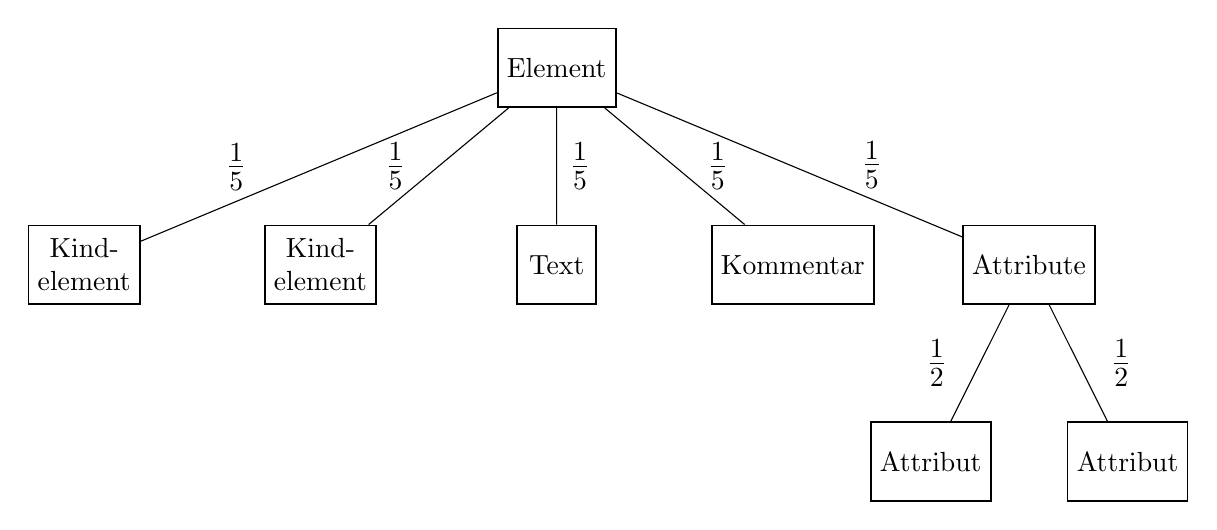
\begin{tikzpicture}[level distance=2.5cm,
  level 1/.style={sibling distance=3cm},
  level 2/.style={sibling distance=2.5cm},
  element/.style={draw=black, fill=white, semithick, minimum size=10mm, align=center},
  attribute/.style={ draw=red, fill=white, semithick, minimum size=7mm, align=center},
  textnode/.style={ draw=black, fill=white, semithick, minimum size=7mm, align=center}]
  \node [element](Root){Element}
    child {node [element]{Kind-\\element}
      edge from parent node[left,font = \Large, outer sep=.80cm]{ \( \frac{1}{5} \)}
    }
    child {node [element]{Kind-\\element}
      edge from parent node[left,font = \Large, outer sep=.30cm]{ \( \frac{1}{5} \)}
    }
    child {node [element]{Text} edge from parent node[right,font = \Large, outer sep=0.5mm]{ \( \frac{1}{5} \)}}
    child {node [element]{Kommentar} edge from parent node[right,font = \Large, outer sep=.30cm]{ \( \frac{1}{5} \)}}
    child {node [element]{Attribute}
      child {node [element]{Attribut} edge from parent node[left,font = \Large, outer sep=.30cm]{ \( \frac{1}{2} \)}}
      child {node [element]{Attribut} edge from parent node[right,font = \Large, outer sep=.30cm]{ \( \frac{1}{2} \)}}
      edge from parent node[right,font = \Large, outer sep=.80cm]{ \( \frac{1}{5} \)}
    };
\end{tikzpicture}